%----------------------------------------------------------------------------------------
%	PACKAGES AND OTHER DOCUMENT CONFIGURATIONS
%----------------------------------------------------------------------------------------

\documentclass[paper=a4, fontsize=11pt]{scrartcl} % A4 paper and 11pt font size
\usepackage[bottom=1.2in]{geometry}

\usepackage[T1]{fontenc} % Use 8-bit encoding that has 256 glyphs
\usepackage{fourier} % Use the Adobe Utopia font for the document - comment this line to return to the LaTeX default
\usepackage[english]{babel} % English language/hyphenation
\usepackage{amsmath,amsfonts,amsthm} % Math packages

\usepackage{sectsty} % Allows customizing section commands
\allsectionsfont{ \rmfamily\scshape} % Make all sections centered, the default font and small caps

\usepackage{fancyhdr} % Custom headers and footers
\pagestyle{fancyplain} % Makes all pages in the document conform to the custom headers and footers
\fancyhead{} % No page header - if you want one, create it in the same way as the footers below
\fancyfoot[L]{} % Empty left footer
\fancyfoot[C]{} % Empty center footer
\fancyfoot[R]{\thepage} % Page numbering for right footer
\renewcommand{\headrulewidth}{0pt} % Remove header underlines
\renewcommand{\footrulewidth}{0pt} % Remove footer underlines
\setlength{\headheight}{13.6pt} % Customize the height of the header

\numberwithin{equation}{section} % Number equations within sections (i.e. 1.1, 1.2, 2.1, 2.2 instead of 1, 2, 3, 4)
\numberwithin{figure}{section} % Number figures within sections (i.e. 1.1, 1.2, 2.1, 2.2 instead of 1, 2, 3, 4)
\numberwithin{table}{section} % Number tables within sections (i.e. 1.1, 1.2, 2.1, 2.2 instead of 1, 2, 3, 4)

\setlength\parindent{0pt} % Removes all indentation from paragraphs - comment this line for an assignment with lots of text

\usepackage[margin=2cm]{caption}
\usepackage{listings}
\usepackage{subcaption}
\usepackage{graphicx}
\newcommand{\aat}{\textbf{AAT}}
\newcommand{\hit}{\textbf{Hit Time}}
%----------------------------------------------------------------------------------------
%	TITLE SECTION
%----------------------------------------------------------------------------------------

\newcommand{\horrule}[1]{\rule{\linewidth}{#1}} % Create horizontal rule command with 1 argument of height

\title{	
\normalfont \normalsize 
\textsc{School of Physics, Georgia Institute of Technology } \\ [25pt] % Your university, school and/or department name(s)
\horrule{0.5pt} \\[0.4cm] % Thin top horizontal rule
\huge RPC-Based Proxy Server \\ % The assignment title
\horrule{2pt} \\[0.5cm] % Thick bottom horizontal rule
}

\author{Group member : \\
\\
 Xiong Ding 902934749 \\ 
 Yuebin Zhou 903005133
} % Your name

\date{\normalsize\today} % Today's date or a custom date

\begin{document}

\maketitle % Print the title

%----------------------------------------------------------------------------------------
%	part 1
%----------------------------------------------------------------------------------------

\section{Introduction}

\section{Cache Design}

Cache is implemented by the combination of \textbf{Hash table} 
and \textbf{doubly linked list}. Each hash entry is 
a tuple \textbf{<URL, node*>}, where the node pointer points to a node
in the doubly linked list (cache list). Each node is a structure
containing the URL and the corresponding web page content.

\vspace{0.5em}

We use the C++ STL container \textbf{std::unordered\_map} to hold the 
hash table. The searching operation in the unordered\_map
has an average complexity of $O(1)$, and the worst case is $O(N)$. Doubly
linked list is used to hold the cached web pages. We insert new nodes
to the head, and remove nodes from the tail. Different cache policies will
implement different rules to manipulate this list, and insert and
delete operations has complexity $O(1)$.

\vspace{0.5em}

The cache class can support two different operations: \textbf{get()} and
\textbf{put()}. whenever there comes a URL, \textbf{get()} will try to look
up the hash table, if the corresponding entry is found, then the web page
content would be returned. 
\textbf{get()} may also modify the node list to reflect recent access
(only for LRU policy). On the other hand, \textbf{put()} function is
responsible for inserting new node to list and deleting nodes if the
total size of cache goes beyond the limits. Therefore, different cache 
policies only need to implement different \textbf{get()} and 
\textbf{put()}, 
such that the interface keeps uniform.

\section{Cache Policies}

\subsection{LRU}
The Least Recent Used policy will keep track of the access order 
of cache list. In our implementation, the closer to the list head, 
the fresher of the web page contained in this node. So every time 
there is a cache hit, the corresponding cache node will be moved to
the head. If the cache is full, the nodes closest to the tail will
be removed first.
\begin{itemize}
\item \textbf{Pros:} LRU can enhance locality. Recently visited websites
are likely to be visited again.
\item \textbf{Cons:} Performance issue: every lookup of the cache needs
to update the double linked cache list no matter it is a hit or
miss.
\end{itemize}

\subsection{Random}
Random policy evicts the cache entry randomly When the total cache 
size exceeds the maximal size. It can be implemented by a random
number generator to choose the replace cache entry.
\begin{itemize}
\item \textbf{Pros:} It will not result in extremely bad performance.
for some special
 patterns, because the eviction decision is not based on the 
access pattern; thus, it has similar performance for all kinds of patterns.
\item \textbf{Cons:} It has higher rates compared with other cache 
policies which take account of access pattern like LRU, because users
are likely to browse a few web pages repeatedly.
\end{itemize}

\subsection{FIFO}
The ``first in first out'' policy will evicts the entry that was put 
into the cache earliest. Cache entries are always inserted at the tail
of the cache container, and evicted from the head of the cache container.
\begin{itemize}
\item \textbf{Pros:} Usually, the oldest entry in the cache is least
likely to be accessed again. FIFO reflects the ``age'' of each cache entry, 
and evicts the oldest page, so it has relatively good performance compared
to random policy.
\item \textbf{Cons:} In some cases, the oldest cache may be accessed again,
such as browsing a few web pages in a circular manner, so there is a large 
number of cache misses. 
\end{itemize}

\section{Evaluation Metrics}

\section{Workloads Generation}

\section{Experiment Description}

\section{Experimental Results \& Analysis}
\begin{figure}[h]
  \centering
  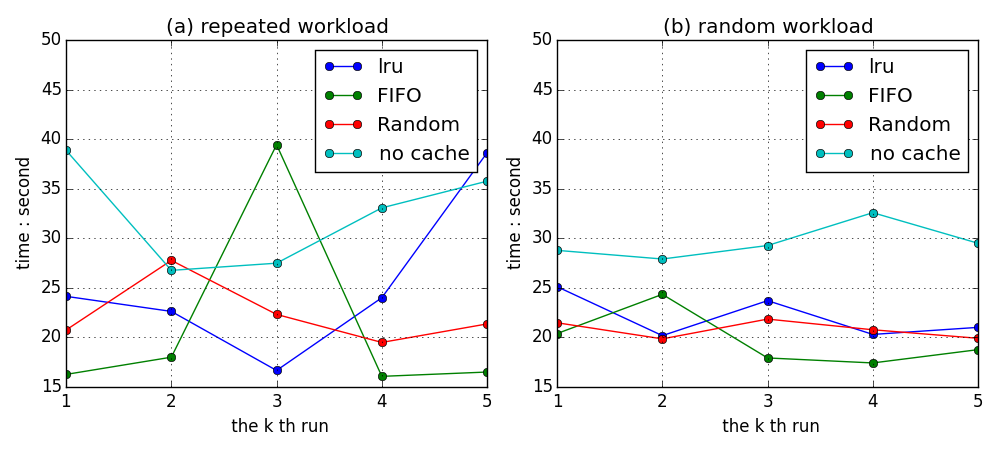
\includegraphics[width=\textwidth]{../data/time512k}
  \caption{cache size = 512k}
  \label{fig:time512k}
\end{figure}
\begin{figure}[h]
  \centering
  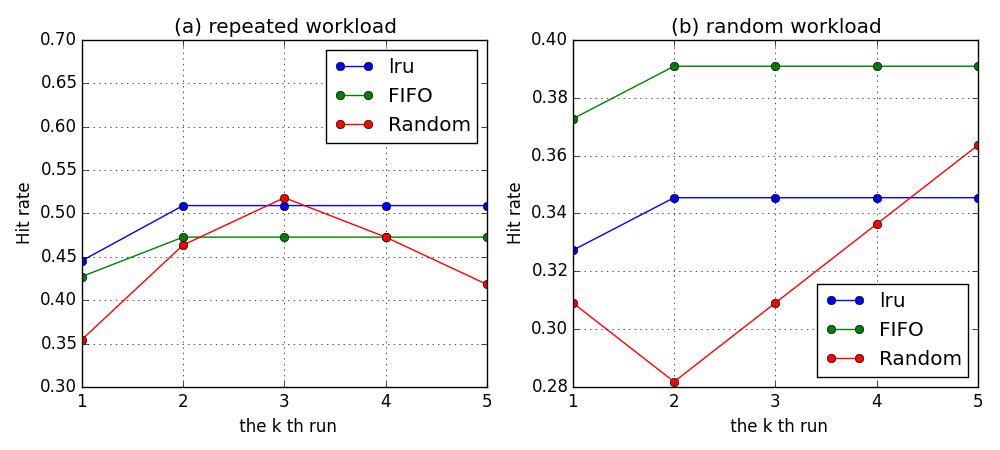
\includegraphics[width=\textwidth]{../data/hit512k}
  \caption{cache size = 512k}
  \label{fig:hit512k}
\end{figure}
\begin{figure}[h]
  \centering
  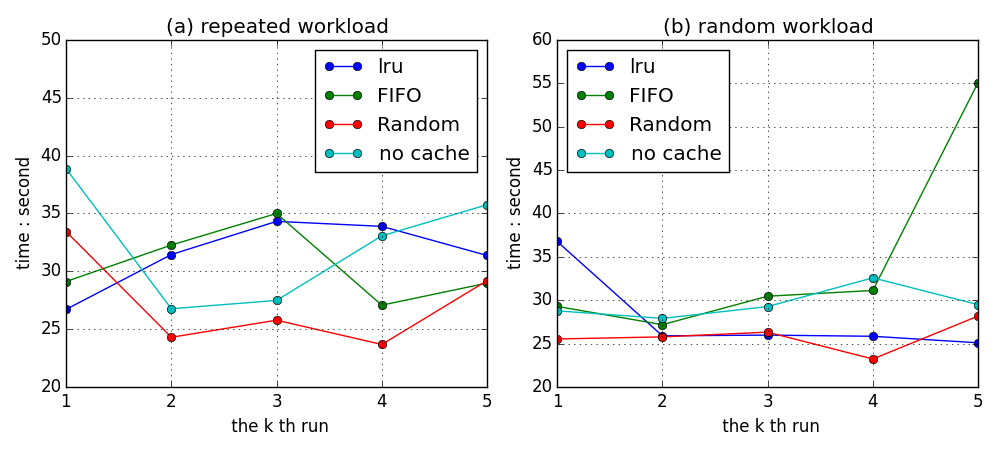
\includegraphics[width=\textwidth]{../data/time256k}
  \caption{cache size = 256k}
  \label{fig:time256k}
\end{figure}
\begin{figure}[h]
  \centering
  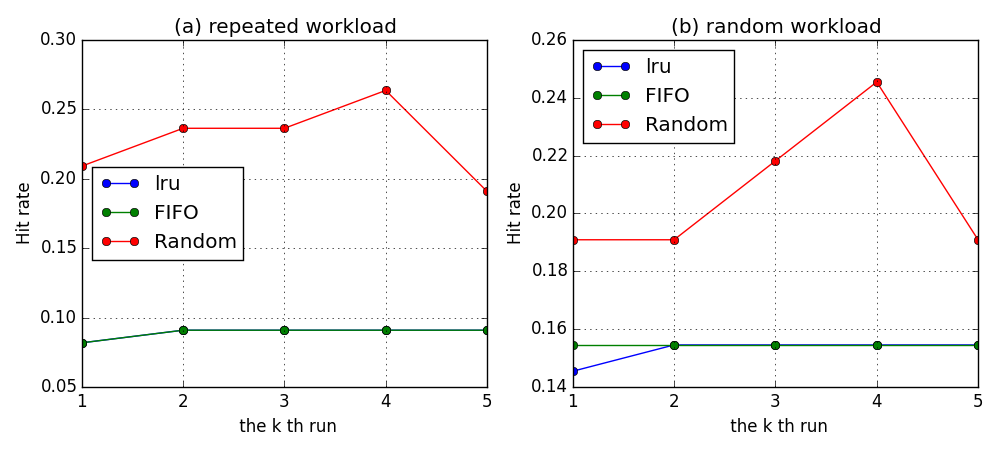
\includegraphics[width=\textwidth]{../data/hit256k}
  \caption{cache size = 256k}
  \label{fig:hit256k}
\end{figure}
\begin{figure}[h]
  \centering
  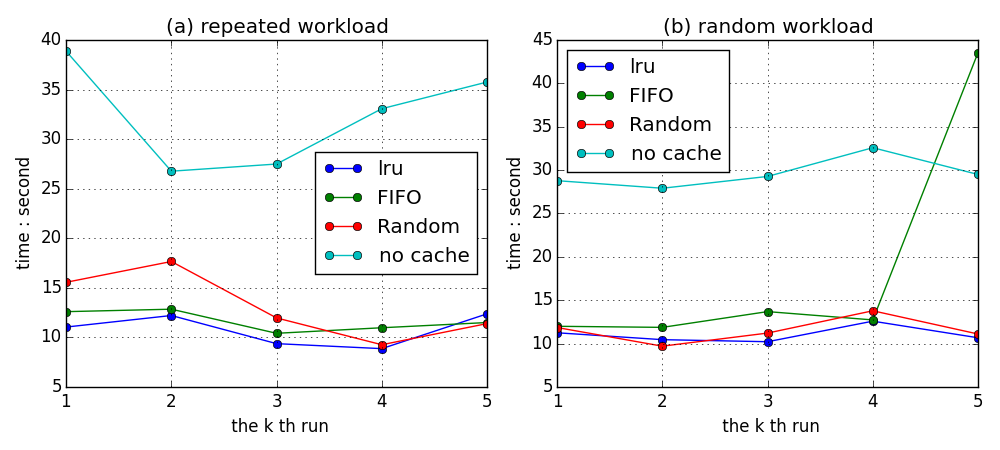
\includegraphics[width=\textwidth]{../data/time1M}
  \caption{cache size = 1M}
  \label{fig:time1M}
\end{figure}
\begin{figure}[h]
  \centering
  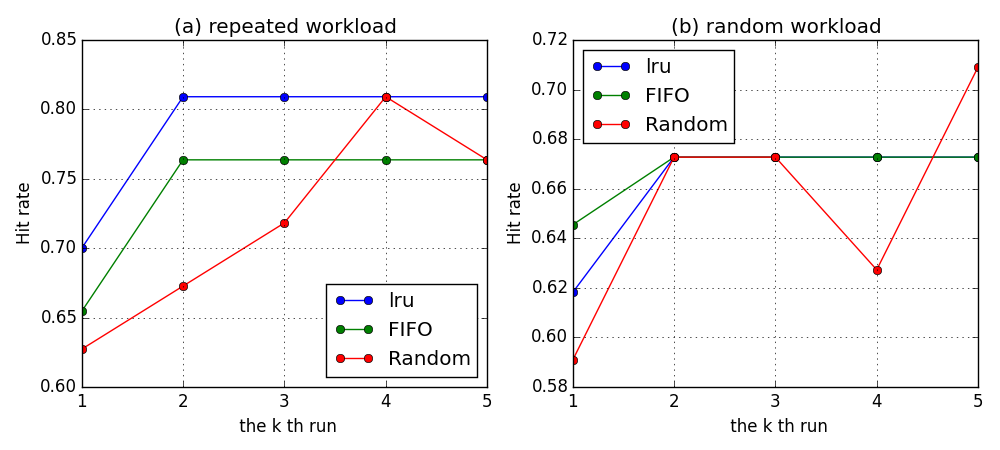
\includegraphics[width=\textwidth]{../data/hit1M}
  \caption{cache size = 1M}
  \label{fig:hit1M}
\end{figure}
\begin{figure}[h]
  \centering
  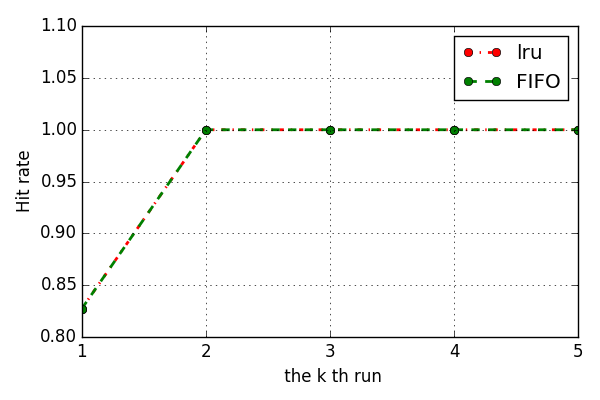
\includegraphics[width=0.7\textwidth]{../data/hit2M}
  \caption{cache size = 2M}
  \label{fig:time2M}
\end{figure}

\section{Conclusion}



\end{document}
